%===============================================================================
% CHAPTER 4: IMPLEMENTATION
%===============================================================================
\chapter{Implementation}
\label{ch:implementation}

\section{Development Environment}
\label{sec:dev-env}

\begin{table}[H]
\centering
\caption{Technology Stack}
\label{tab:tech-stack}
\begin{tabular}{@{}ll@{}}
\toprule
\textbf{Category} & \textbf{Technology} \\
\midrule
Backend Runtime & Node.js (Express 5.2.1) \\
Frontend Framework & React 18.2 (Vite 8.3.5) \\
Database & MongoDB (Mongoose 9.10.1) \\
Blockchain SDK & @hashgraph/sdk (Hedera Testnet) \\
Authentication & JWT (jsonwebtoken), bcrypt \\
Containerization & Docker, Docker Compose \\
Reverse Proxy & Nginx (production frontend) \\
Language & JavaScript (ES2022), JSX \\
Styling & CSS3 (custom properties, component stylesheets) \\
Testing & Node.js built-in test runner \\
\midrule
\end{tabular}
\end{table}

\section{Backend Implementation}
\label{sec:backend-impl}

\subsection{Server Initialization}
\label{sec:server-init}

The \texttt{server.js} entry point configures Express, connects to MongoDB, initializes
the Hedera client, seeds default data, and registers routes.

\begin{lstlisting}[style=codeStyle, caption=Server initialization (excerpt), label=lst:server-init]
const express = require("express");
const cors = require("cors");
const mongoose = require("mongoose");
const { Client, PrivateKey } = require("@hashgraph/sdk");

const app = express();
app.use(cors());
app.use(express.json());

// MongoDB
await mongoose.connect(process.env.MONGO_URI);

// Hedera Client
const client = Client.forTestnet();
client.setOperator(process.env.HEDERA_ACCOUNT_ID, process.env.HEDERA_PRIVATE_KEY);

// Seed default accounts (ADMIN001, VOTER001)
await createDefaultAccounts();

// Routes
app.post("/api/auth/login", login);
app.get("/api/election", getElection);
app.post("/castVote", authenticateToken, requireRole("Voters"), castVote);
// ... admin routes
\end{lstlisting}

\subsection{Authentication \& Authorization}
\label{sec:auth-impl}

JWT-based authentication with role claims:

\begin{lstlisting}[style=codeStyle, caption=JWT middleware, label=lst:jwt-middleware]
const authenticateToken = (req, res, next) => {
  const token = req.headers.authorization?.split(" ")[1];
  if (!token) return res.status(401).json({ error: "Access token required" });

  jwt.verify(token, JWT_SECRET, (err, user) => {
    if (err) return res.status(403).json({ error: "Invalid or expired token" });
    req.voterId = user.sub;
    req.role = user.role;
    next();
  });
};

const requireRole = (role) => (req, res, next) => {
  if (req.role !== role) return res.status(403).json({ error: "Insufficient permissions" });
  next();
};
\end{lstlisting}

\subsection{Vote Casting Endpoint}
\label{sec:vote-endpoint}

The critical \texttt{/castVote} endpoint (lines 290--356 in server.js) implements
the atomic DB+HCS coordination described in Section~\ref{sec:vote-flow}.

\subsection{Admin Endpoints}
\label{sec:admin-endpoints}

Admin-only routes for election management:

\begin{itemize}
    \item \texttt{POST /api/admin/candidates} -- Create candidate with manifesto
    \item \texttt{PUT /api/admin/candidates/:id} -- Update candidate profile
    \item \texttt{PUT /api/admin/candidates/:id/manifesto} -- Replace manifesto array
    \item \texttt{PUT /api/admin/candidates/:id/performance} -- Update performance records
    \item \texttt{POST /api/admin/voters} -- Enroll new voter
    \item \texttt{POST /api/admin/toggle-status} -- Open/close election
    \item \texttt{POST /api/admin/reset} -- Reset all voter participation
    \item \texttt{POST /api/admin/evidence} -- Create evidence document
    \item \texttt{POST /api/admin/issues} -- Create campus issue
    \item \texttt{POST /api/admin/seed-manifesto} -- Reseed demo data
\end{itemize}

\subsection{Data Seeding}
\label{sec:seeding}

\texttt{seedData.js} populates the database with demonstration data:
\begin{itemize}
    \item 3 candidates with detailed manifestos and performance records
    \item 6 campus priority issues with proposed solutions
    \item 8 evidence documents (reports, letters, surveys) with verification status
    \item Performance records for incumbent candidates
\end{itemize}

\section{Frontend Implementation}
\label{sec:frontend-impl}

\subsection{Routing \& Auth State}
\label{sec:routing}

\texttt{App.jsx} manages authentication state and role-based routing:

\begin{lstlisting}[style=codeStyle, caption=App.jsx routing logic, label=lst:app-routing]
function AppRoutes({ auth, onLogout }) {
  const [voterView, setVoterView] = useState(
    () => sessionStorage.getItem("voterView") || "manifesto"
  );

  return (
    <Routes>
      <Route path="/admin" element={
        auth.role === "Admins" ? <AdminConsole /> : <Navigate to="/manifesto" />
      } />
      <Route path="/manifesto" element={
        auth.role === "Voters" ? <ManifestoDashboard /> : <Navigate to="/admin" />
      } />
      <Route path="/vote" element={
        auth.role === "Voters" && voterView === "ballot"
          ? <VoterBooth /> : <Navigate to="/manifesto" />
      } />
      <Route path="*" element={<Navigate to={auth.role === "Admins" ? "/admin" : "/manifesto"} />} />
    </Routes>
  );
}
\end{lstlisting}

\subsection{ManifestoDashboard}
\label{sec:manifesto-dash}

The \texttt{ManifestoDashboard} component (55KB) provides:
\begin{itemize}
    \item \textbf{Candidates Tab:} Card grid with expandable manifesto promises
    \item \textbf{Issues Tab:} Campus priority issues with urgency badges
    \item \textbf{Evidence Tab:} Verified documents with snippet preview
    \item \textbf{Compare Tab:} Side-by-side candidate comparison
    \item \textbf{Proceed to Vote:} Gated navigation to ballot
\end{itemize}

\subsection{VoterBooth}
\label{sec:voter-booth}

The \texttt{VoterBooth} component handles ballot casting:
\begin{itemize}
    \item Candidate selection with radio buttons
    \item Confirmation modal before submission
    \item Loading state during HCS submission
    \item Success screen with transaction ID and HashScan link
\end{itemize}

\subsection{AdminConsole}
\label{sec:admin-console}

The \texttt{AdminConsole} component (22KB) provides tabbed panels:
\begin{itemize}
    \item \textbf{Dashboard:} Real-time stats (total voters, voted, turnout %)
    \item \textbf{Candidates:} CRUD with manifesto/performance editors
    \item \textbf{Voters:} Enrollment with auto-generated passwords
    \item \textbf{Issues:} Campus issue management
    \item \textbf{Evidence:} Document archive with verification status
    \item \textbf{Settings:} Election toggle, voter reset, data reseed
\end{itemize}

\subsection{UI/UX Design System}
\label{sec:design-system}

The implemented interface uses a shared studio-style visual language across the
login, manifesto, and ballot flows. Figure~\ref{fig:ui-login} shows the public
authentication surface, while Figure~\ref{fig:ui-candidate-spec} shows the
candidate specification view used for focused manifesto review.

\begin{figure}[H]
\centering
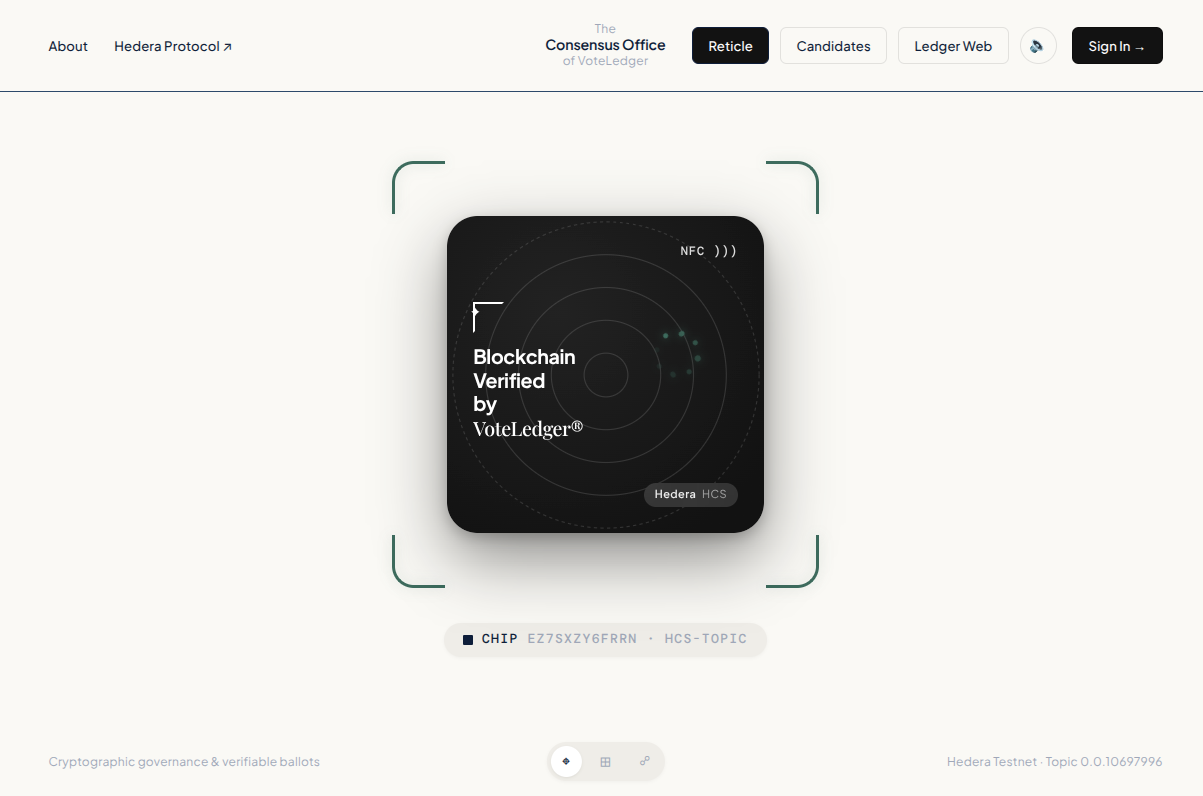
\includegraphics[width=0.92\textwidth]{figures/ui-login.png}
\caption{VoteLedger studio-style login and cryptographic reticle interface}
\label{fig:ui-login}
\end{figure}

\begin{figure}[H]
\centering
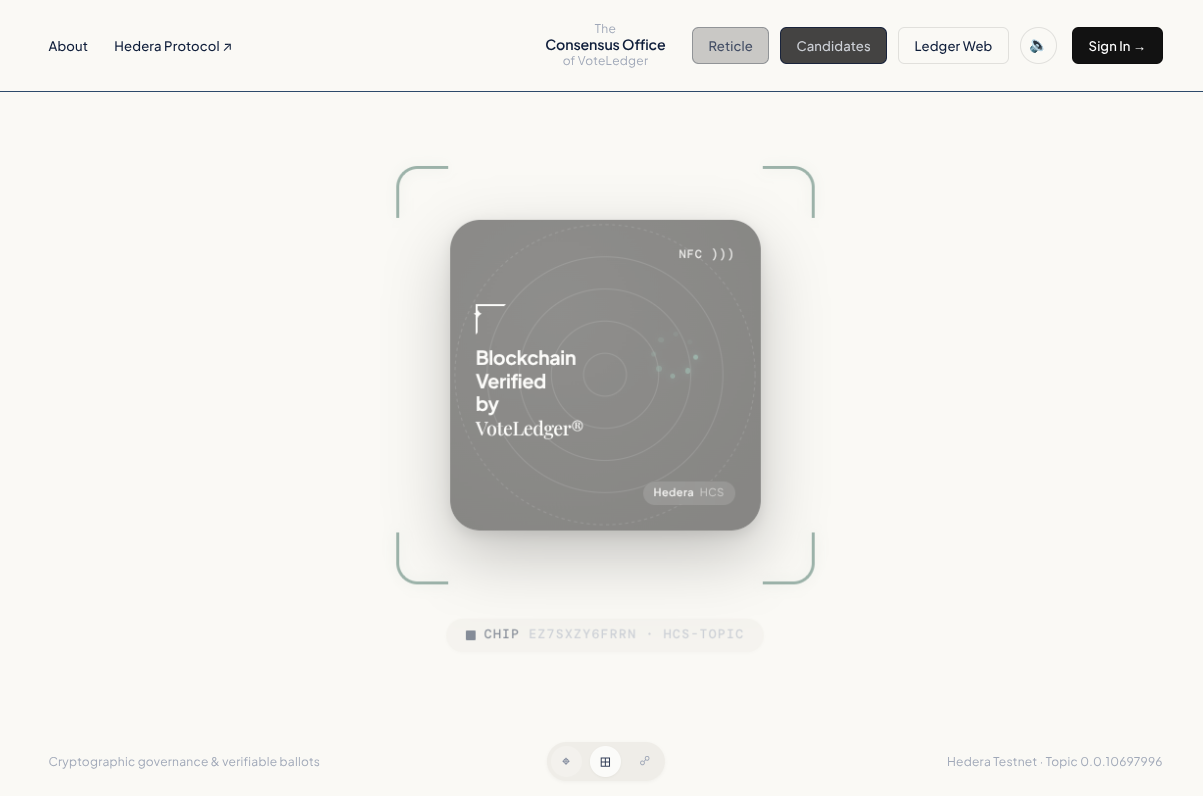
\includegraphics[width=0.92\textwidth]{figures/ui-candidate-spec.png}
\caption{Candidate specification view with detailed manifesto access}
\label{fig:ui-candidate-spec}
\end{figure}

Custom CSS with CSS variables for theming:

\begin{lstlisting}[style=codeStyle, caption=CSS Custom Properties (excerpt), label=lst:css-vars]
:root {
  --color-primary: #1e3a5f;
  --color-primary-light: #2d5a8a;
  --color-accent: #d4a843;
  --color-accent-light: #e8c56d;
  --color-bg: #f8f9fa;
  --color-surface: #ffffff;
  --color-text: #2d3142;
  --color-text-muted: #5a6a80;
  --color-success: #2e7d32;
  --color-error: #c62828;
  --color-warning: #ef6c00;
  --font-family: "Manrope", -apple-system, BlinkMacSystemFont, sans-serif;
  --radius-sm: 4px; --radius-md: 8px; --radius-lg: 12px;
  --shadow-sm: 0 1px 2px rgba(0,0,0,0.05);
  --shadow-md: 0 4px 6px rgba(0,0,0,0.07);
  --shadow-lg: 0 10px 25px rgba(0,0,0,0.1);
}
\end{lstlisting}

Responsive breakpoints: mobile (<640px), tablet (640--1024px), desktop (>1024px).

\section{Blockchain Integration}
\label{sec:blockchain-impl}

\subsection{Hedera Client Configuration}
\label{sec:hedera-client}

The Hedera client is initialized inline in \texttt{server.js}:

\begin{lstlisting}[style=codeStyle, caption=Hedera client setup, label=lst:hedera-client]
const { Client, PrivateKey, TopicMessageSubmitTransaction } = require("@hashgraph/sdk");

let client;
if (process.env.HEDERA_NETWORK === "localnet") {
  client = Client.forLocalnet();
} else {
  client = Client.forTestnet();
}

const privateKey = process.env.HEDERA_PRIVATE_KEY.trim();
client.setOperator(
  process.env.HEDERA_ACCOUNT_ID.trim(),
  privateKey.startsWith("0x") || privateKey.length === 66
    ? PrivateKey.fromStringECDSA(privateKey)
    : PrivateKey.fromString(privateKey)
);

const topicId = process.env.HCS_TOPIC_ID;
\end{lstlisting}

\subsection{Message Format}
\label{sec:msg-format}

Votes are submitted as JSON messages to the HCS topic:

\begin{lstlisting}[style=codeStyle, caption=Vote message format, label=lst:vote-msg]
{
  "candidateId": "1",
  "timestamp": "2026-10-28T14:30:00.000Z"
}
\end{lstlisting}

\subsection{Mirror Node Query}
\label{sec:mirror-query}

Results are aggregated by querying mirror nodes:

\begin{lstlisting}[style=codeStyle, caption=Mirror node aggregation, label=lst:mirror-query]
async function fetchVoteTally(topicId) {
  const url = `https://testnet.mirrornode.hedera.com/api/v1/topics/${topicId}/messages`;
  const response = await fetch(url);
  const data = await response.json();

  const votes = data.messages.map(msg => JSON.parse(Buffer.from(msg.message, "base64").toString()));
  return votes.reduce((acc, v) => {
    acc[v.candidateId] = (acc[v.candidateId] || 0) + 1;
    return acc;
  }, {});
}
\end{lstlisting}

\section{Testing Strategy}
\label{sec:testing}

\begin{itemize}
    \item \textbf{Automated tests:} Seven Node.js tests covering authentication and Hedera error handling
    \item \textbf{Integration testing:} Requires a configured MongoDB instance and funded Hedera testnet account
    \item \textbf{E2E manual testing:} The voter journey is documented as a checklist; execution evidence must be attached for submission
    \item \textbf{Load testing:} No reproducible load-test harness is currently included in the repository
\end{itemize}
